\chapter{Introducing MATSim}
\label{ch:introducing}
% ##################################################################################################################
\hfill \textbf{Author:} Kay W. Axhausen, Andreas Horni, ...

\begin{center} 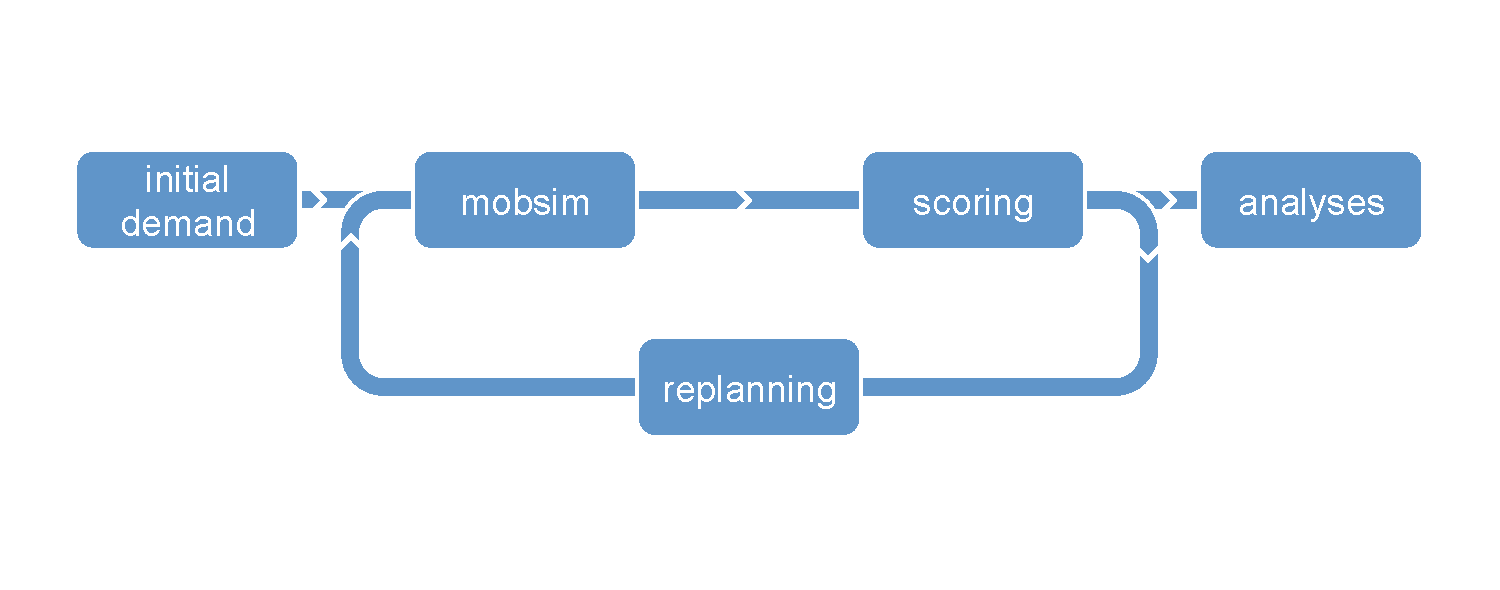
\includegraphics[width=0.7\textwidth, angle=0]{figures/matsimcycle.pdf} \end{center}

% ##################################################################################################################

%\ah{The development of the multi-agent transport simulation MATSim \citep[][]{MATSIM-T_Webpage_2014, BalmerEtAl_TRR_2006} has started approximately a decade ago as a collaborative effort of Prof.\ Nagel (now: TU Berlin) and Prof.\ Axhausen (ETH Zurich). It has its roots in \citet[][]{Axhausen_PhDThesis_1988} and in the transport simulation TRANSIMS \citep[][]{RaneyEtAl_LNCS_2002}, which was developed by Prof.\ Nagel as research team leader at the Los Alamos National Laboratory.}

% ##################################################################################################################
\section{How It Started}
The multi-agent transport simulation MATSim \citep[][]{MATSIM-T_Webpage_2014} started with the wish of Prof. Nagel, then at ETH Zurich, to improve on his work with and for the TRANSIMS project \citep[][]{SmithEtAl_NTRPAC_1995} and to make the resulting code open-source. His background in traffic flow was then complemented with experience in the agent-based modeling of travel demand, when after Prof. Nagel departure to Berlin in 2004 Prof. Axhausen joined the effort in earnest. 

It is this merger of two, actually three large and old streams of research, which has made the system unique from the start: microscopic description of demand by tracing the daily schedule and the decisions involved of the agents modeled, integral microscopic simulation of the resulting traffic flows and the resulting congestion, optimization of the experienced utilities of the whole schedule through the co-evolutionary search for the resulting equilibrium or steady state (see Section~\ref{sec:co-ev}). The robustness of this framework for the description of all congested spatial behaviors became clear, as the development progressed to include the congestion inside facilities and buildings or as parking was added. 

Agent-based modeling had been the basis of traffic flow simulation from the start in the 1970’s, e.g., \citet[][]{Wiedemann_PhDThesis_1974} or \citet[][]{Seddon_Simulation_1972}, but the work on traffic flow limited itself to individual links or small sequences of links and could therefore not address equilibrium as the aggregate assignment models could do from the 1970’s onward \citep[see][]{OrtuzarWillumsen_2011}. The expansion to whole and large networks came with the increasingly more powerful computers in the 1980’s and fast and accurate enough flow models (e.g. \citet[][]{NagelSchreckenberg_JdPI_1992, Schwerdtfeger_VolmulerHamerslag_1984, Daganzo_TransResPartB_1994}, but these agent-based simulations were not used to find an equilibrium at first. 

Agent-based modeling of travel demand had been developed in Germany \citep[][]{AxhausenHerz_JTE_1989}, but then also in English speaking countries after the seminar book of \citet[][]{JonesEtAl_1983}. While the Anglophone authors focused on sample enumeration methods to estimate the total demand with their agent-based demand models (see \citet[see][]{BradleyBowman_TRBTDF_2006} for the North American, mostly discrete choice model based, developments, and \citet[][]{ArentzeTimmermans_2000} for an alternative Dutch approach), the simpler German approach was linked with an integral mesoscopic traffic flow simulation in \citet[][]{Axhausen_PhDThesis_1988}, but not used for equilibrium search. It had already a simple description of the total utility of the daily schedule.

Nash-equilibrium like approaches had been developed in transport assignment since the seminal \citet[][]{Wardrop_PICE_1952} paper, these aggregate flow based approaches were expanded to account for perception errors of the user and for the social optimum \citep[see][]{DaganzoSheffi_TransScience_1977}, but their reformulation for an disaggregate agent-based solution had to wait until the late 1990’s with \citet[][]{Gawron_IJMPC_1998} and TRANSSIMS \citep[][]{SmithEtAl_NTRPAC_1995}. These approaches translated the logic of genetic algorithms into co-evolutionary search scheme, which efficiently identified the optima of each agent’s daily schedule.

At the end of 1990’s the scene was set for a merger of these strands into a computationally efficient, modular and open-source software enabling further development on travel behavior, network response and efficient computation. 

As shown on the web page \citep[][]{MATSIM-T-Scenarios_Webpage_2015} and detailed in Chapter \ref{ch:scenarios}, MATSim has been applied by local research groups world-wide for several different regions.

% ##################################################################################################################
\section{In Brief}
MATSim is an activity-based, extendable, multi-agent simulation toolkit implemented with the programming language \gls{java}. It is open-source and can be downloaded freely at \citep[][]{MATSIM-T_Webpage_2015, SourceForge_Webpage_2015}. The framework is especially designed for large-scale scenarios, meaning that, the features of all models are generally stripped down to efficiently handle the targeted functionality, where emphasis has been also been laid on parallelization \citep[e.g.,][]{Dobler_TechRep_IVT_2011, Charypar_PhDThesis_2008}. For the network loading simulation, for example, a queue-based model is implemented, leaving out the very complex car-following behavior (see Section~\ref{sec:trafficflowmodel}).

For now, MATSim is conceptually designed to model a \emph{single day}, a common unit of analysis for activity-based models (see, for example, the review in \citet[][]{Bowman_TEC_2009_1}). In other words, MATSim is basically a cross-sectional model. Nevertheless, in principle a longitudinal model could be implemented \citep[][]{HorniEtAl_TechRep_IVT_2012_a}.

As shown in Section~\ref{sec:co-ev}, MATSim is based on a co-evolutionary principle. While being in a competition for space-time slots on the transportation infrastructure with all the other agents, every agent iteratively optimizes its daily activity schedule. This is done by running through the \index{MATSim loop} as depicted in Figure \ref{fig:matsimcycle}. 

MATSim starts with an initial demand, which is composed of the study area population's daily activity chains. The modeled persons are called agents in MATSim. The activity chains are usually derived from empirical data. A variety of data is suitable as can be seen in the scenarios chapter. During the iterations this initial demand is optimized, where every agent possesses a memory of a fixed number of day plans, where each plan is composed of a daily activity chain and an associated utility value (in MATSim called \emph{plan score}).

In every iteration, prior to the simulation of the network loading in the MATSim \gls{mobsim} \citep[e.g.,][]{Cetin_PhDThesis_2005} (\emph{execution}), every agent selects a plan from its memory. This selection is dependent on the plan utility. A certain share of the agents $\varphi$ (usually around 10$\%$) is allowed to clone the selected plan and modify this clone (\emph{replanning}). For the method of successive averages (MSA) usually a decreasing share of travelers is reallocated to a new route to avoid oscillations. For MATSim, it has been shown that a variable replanning share can be productive as well and \emph{``increases overall performance of the system by a factor of three or more''} \citep[][p.7f]{CharyparEtAl_IATBR_2006}. For the network loading microsimulation step multiple simulations are available and configurable \citep[][p.10f]{HorniEtAl_TechRep_IVT_2011_a}. 

Plan modification is implemented in the \emph{replanning} modules. Four choice dimensions are usually considered in standard MATSim for now: time choice \citep[][]{BalmerEtAl_Timmermans_2005}, route choice \citep[]{LefebvreBalmer_STRC_2007}, mode choice, and destination choice. Further choices such as activity adding or dropping or parking and group choices are currently researched. % Siehe Tabelle MATSim-Präsentationen Prof.\ Axhausen.
MATSim replanning offers different strategies to adapt plans ranging from random mutation to approximate suggestions, to best response answers, where in every iteration the currently optimal choice is searched. Usually, routing and destination choice are best response modifications, where time choice and mode choice are random mutations. 

The initial day chains do not need to be designed overly careful for the choice dimensions that are included in the optimization process. Plausible values just speed-up the optimization process. 

If an agent ends up with too many plans (configurable), the plan with the lowest score (configurable) is removed from the memory of this agent. The agents, which have not undergone replanning select between existing plans. The selection model is configurable; in many MATSim investigations, a model that generates a logit distribution for plan selection is used.

An iteration is completed by evaluating the agent's day described by the selected day plans (\emph{scoring}). The applied utility function is described in detail in Chapter \ref{ch:scoring}.

The iterative process is repeated until the average population score stabilizes, where the definition of the stopping criterion is subject of ongoing research initialized by \citet[][]{Meister_PhDThesis_2011, NagelFloetteroed_IATBR_2009}. The typical score development curve (Figure~\ref{fig:scoreprogress}, taken from \citet[][]{HorniEtAl_TRR_2009}) has the form of the common evolutionary optimization progress \citep[][p.]{EibenSmithJE_2003}.

MATSim offers considerable customizability through its modular design approach. Although, replacing core modules, such as the network loading simulation is associated with a substantial effort \citep[][Section 2.4]{MATSim_Userguide_2014} in principle every module of the framework can be replaced. MATSim modules are described in Chapter \ref{ch:modules} and following.

MATSim is heavily-based on events. Every action in the simulation generates an event. These events can be aggregated to evaluate any measure with the desired resolution. The event architecture is detailed in Section~\ref{sec:events}.

% ------------
\createfigure%
{MATSim Cycle}%
{MATSim Cycle}%
{\label{fig:matsimcycle}}%
{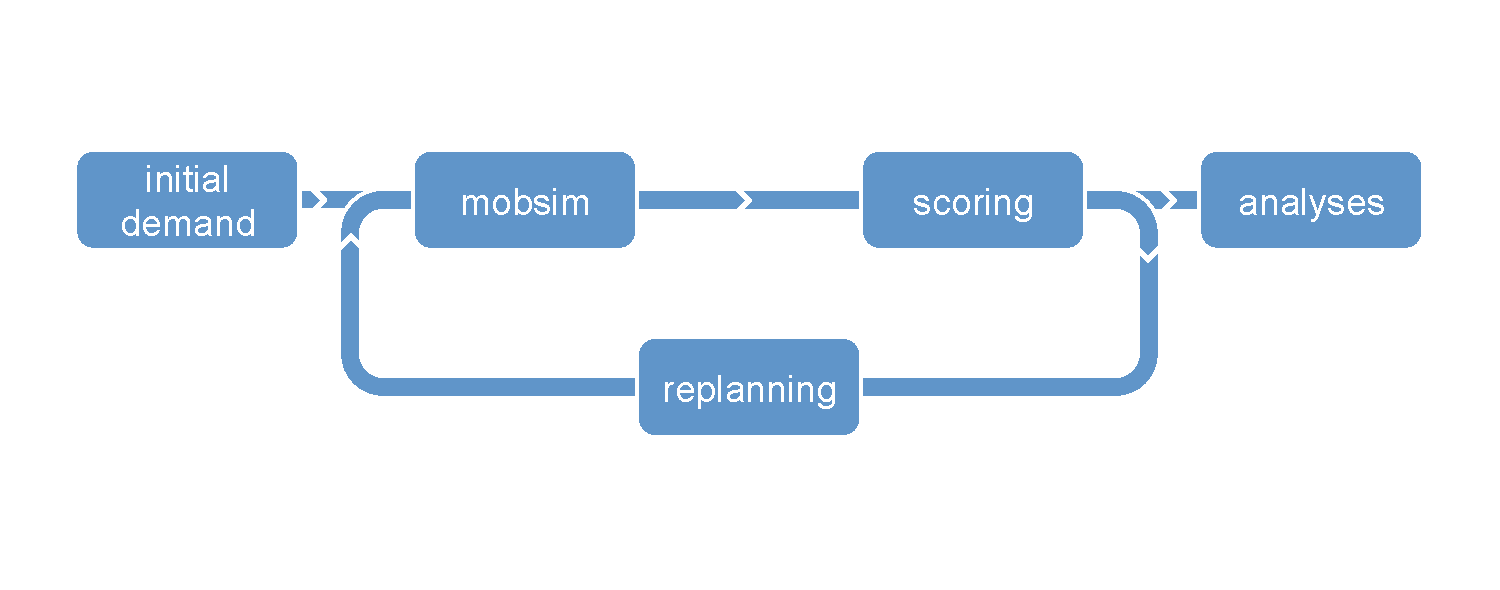
\includegraphics[width=0.99\textwidth, angle=0]{figures/matsimcycle.pdf}}%
{}
% ------------
% ------------
\createfigure%
{Typical Score Progress}%
{Typical Score Progress}%
{\label{fig:scoreprogress}}%
{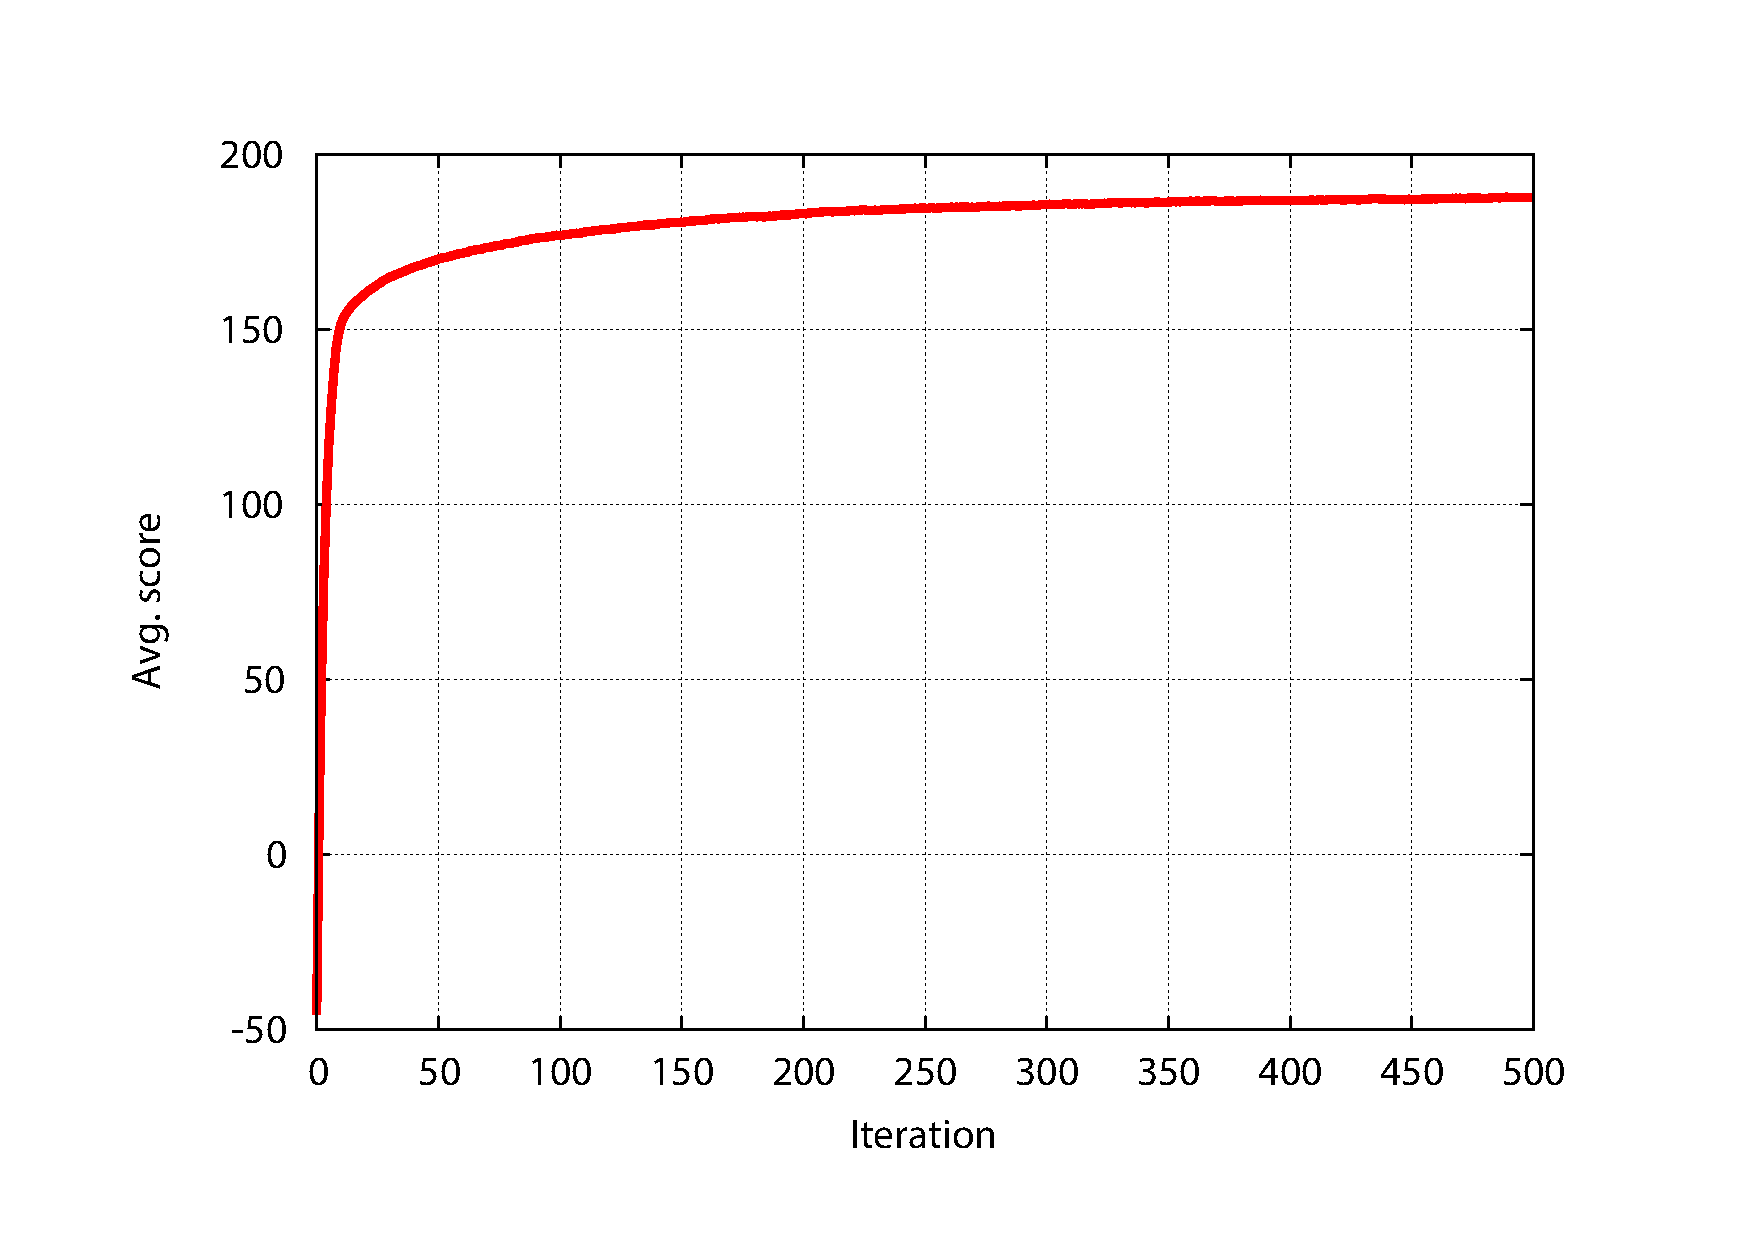
\includegraphics[width=0.99\textwidth, angle=0]{using/figures/scores.pdf}}%
{}
% ------------

% ##################################################################################################################
\section{MATSim's Traffic Flow Model}
\label{sec:trafficflowmodel}
MATSim provides two internal mobility simulations (called \emph{mobsims}): \emph{Qsim} and \emph{JDEQSim}. \emph{queueSimulation} has been deleted recently. Furthermore, external mobility simulations can be plugged in. Some years ago the DEQSim written in C++ and described by \citet[][]{Charypar_PhDThesis_2008, CharyparEtAl_TRR_2007, CharyparEtAl_TRB_2009, CharyparEtAl_WCTRS_2007} was plugged into MATSim and frequently used. The multi-threaded qsim is the default mobsim \citep[][]{MATSim_Userguide_2014}. % commit 29999 michaz

\citet[][]{CharyparEtAl_TRB_2009} distinguishes between 
\begin{compactitem}
\item physical microsimulation models, featuring detailed car following models,
\item cellular automata, in which roads are discretized in cells,
\item queue-based simulations, where traffic dynamics are modeled with waiting queues,
\item mesoscopic models, using aggregates to determine travel speeds, and
\item macroscopic models, based on flows rather than single traveler units (e.g., cars).
\end{compactitem}

As MATSim is designed for large-scale scenarios it adopts an efficient queue-based approach (see Figure \ref{fig:queue}). A car entering a network link (i.e., a road segment) is added to the tail of the waiting queue. It remains there until the time for traveling the link with free flow has passed and until he or she is the head of the waiting queue and until the next destination link allows entering. The approach is very efficient, but clearly it comes at the price of reduced resolution, i.e., car following effects are not captured.   

For computational reasons the waiting-queue approach is combined with an event-based update step \citep[][]{CharyparEtAl_TRB_2009}. In other words, there is no time-step-based updating process of any agent in the scenario. Instead agents are only touched if they actually require an action. For example. during the time an agent needs to pass a link (i.e., he is waiting in the queue), he does not need to be processed. Triggering of update events is managed by a global scheduler.

The MATSim traffic flow model, and as we will see also gridlock modeling, is heavily based on the two measures: storage capacity and flow capacity. Storage capacity defines the number of cars fitting onto a network link. It is a physical property and thus essentially fixed in the simulation. For sample scenarios, however, it needs to be scaled.

Flow capacity gives the outflow capacity of a link, i.e., how many travelers can leave the respective link. It is an individual measure per link. In the earlier DEQSim and in the current JDEQSim the inflow capacity can be specified in addition to capture breakdowns at link inlets \citep[][p.99]{Charypar_PhDThesis_2008}. The many simulation experiments with qsim (and queueSimulation) have shown, that neglecting inflow capacity has not a substantial effect but further reduces model complexity. 

This basic traffic flow model has been extended with various modules: signals and multiple lane modeling have been added (Chapter~\ref{ch:signalslanes}), backward-moving gaps as realized by \citep[][]{Charypar_PhDThesis_2008} are included in qsim. Interactions between different modes are described in Chapter~\ref{ch:multimodalsim}. Limitations of the traffic flow model concern link dynamics (in particular overtaking and slow drivers) and intersection dynamics (in particular turn restrictions not explicitly modeled in the network). 

\createfigure%
{Traffic Flow Model}%
{Traffic Flow Model}%
{\label{fig:queue}}%
{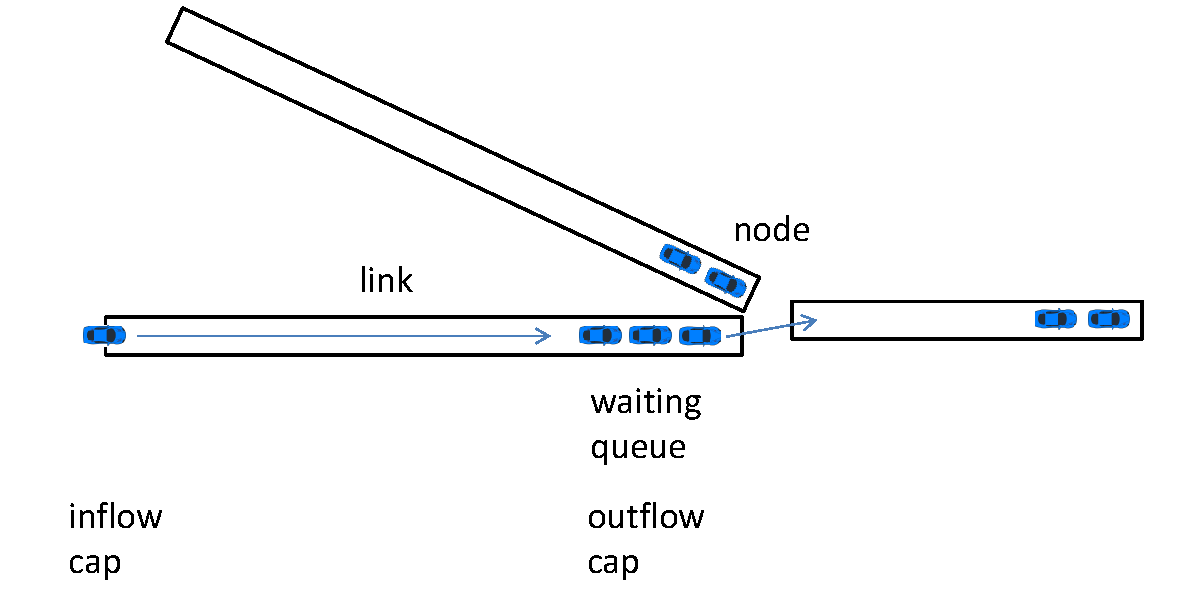
\includegraphics[width=0.99\textwidth, angle=0]{using/figures/queue.pdf}}%
{}


% ##################################################################################################################
\section{MATSim's Co-Evolutionary Algorithm}
\label{sec:co-ev}
As illustrated in Figure \ref{fig:ea}, the MATSim equilibrium is searched by a \emph{\index{co-evolutionary algorithm}}. These algorithms co-evolve different species subject to interaction (e.g., competition). In MATSim, the individuals are represented by the plans of a person, where a person represents a species. By applying the co-evolutionary algorithm, optimization is performed in terms of agents' plans. Eventually, an equilibrium is reached subject to constraints, where the agents cannot further improve their plans unilaterally. When speaking in strict terms, there is a difference between application of an evolutionary algorithm and a \emph{co}-evolutionary algorithm. An evolutionary algorithm would lead to a system optimum as optimization is applied with a global (or population) fitness function. The co-evolutionary algorithm instead leads to a user equilibrium as optimization is performed in terms of \emph{individual} utility functions and within an agent's set of plans. At the moment, the MATSim co-evolutionary algorithm only includes mutation; recombination may come into play when joint day plans of family members, for example, are included in the future.

% ------------
\createfigure%
{Adopting a Co-Evolutionary Algorithm in MATSim}%
{Adopting a Co-Evolutionary Algorithm in MATSim}%
{\label{fig:ea}}%
{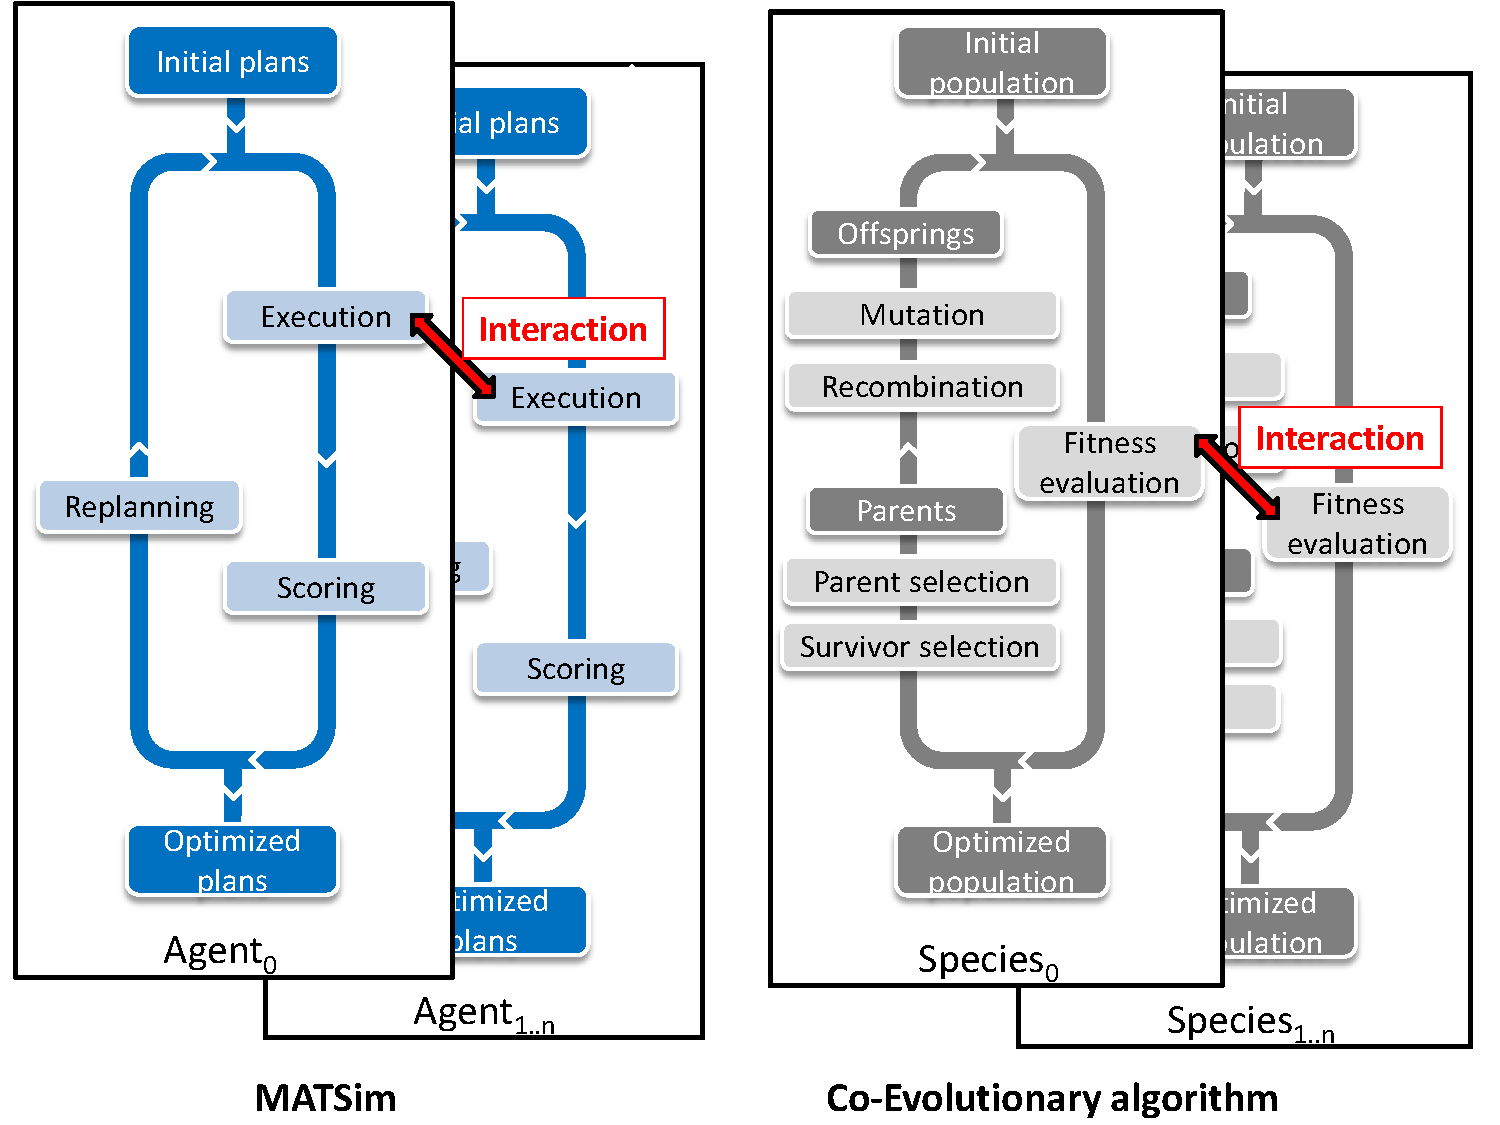
\includegraphics[width=0.99\textwidth, angle=0]{using/figures/MATSimVSea.pdf}}%
{}

% ------------

% ##################################################################################################################
